\documentclass{ximera}

\newcommand{\RR}{\mathbb R}
\renewcommand{\d}{\,d}
\newcommand{\dd}[2][]{\frac{d #1}{d #2}}
\renewcommand{\l}{\ell}
\newcommand{\ddx}{\frac{d}{dx}}
\newcommand{\dfn}{\textbf}
\newcommand{\eval}[1]{\bigg[ #1 \bigg]}


\outcome{Interpert the product of rate and time as area.}
\outcome{Approximate position from velocity.}
\outcome{Recognize Riemann sums.}



\title[Dig-In:]{Relating velocity and position, antiderivatives and areas}


\begin{document}
\begin{abstract}
We see a connection between approximating antiderivatives and approximating areas. 
\end{abstract}
\maketitle

A central theme of this course has been that we can often gain a
better understanding of a function by looking at its derivative, and
then working backwards.  This has been our approach to max/min
problems, curve sketching, linear approximation, and so on.  So
antiderivatives have really been important to us all along. We have a
geometric interpretation of the derivative as the slope of a tangent
line at a point.  We have not yet found a geometric interpretation of
antiderivatives.


\section{More than one perspective}

We'll start with a question:

\begin{question}
   Suppose you are in slow traffic moving at $4$ \textrm{mph} from
   $2$pm to $5$pm.  How far have you traveled?
   \begin{prompt}
     \[
     \answer{12}\ \text{miles}.
     \]
   \end{prompt}
   \begin{hint}
    A fancy way of saying this is that $f$ is a line of slope $4$, and
    we are looking for the rise corresponding to a run of $5-2= 3$.
   \end{hint}
  \end{question}

Now we move to a seemingly unrelated question:

  \begin{question}
    What is the area of the region bounded by the graph of $f(x) = 4$, the horizontal
    axis, and the vertical lines $x=2$ and $x=5$?
    \begin{prompt}
      \[
      \answer{12}
      \]
    \end{prompt}
    \begin{hint}
      \begin{image}
  \begin{tikzpicture}[
      declare function = {f(\x) = 4;} ]
	\begin{axis}[
            domain=-.2:7, xmin =-.2,xmax=7,ymax=5,ymin=-.2,
            width=4in,
            height=2in,
            xtick={2,5}, 
	   ytick={4},
            xticklabels={$2$,$5$},
            yticklabels={$4$},
            axis lines=center, xlabel=$x$, ylabel=$y$,
            every axis y label/.style={at=(current axis.above origin),anchor=south},
            every axis x label/.style={at=(current axis.right of origin),anchor=west},
            axis on top,
          ]
          \addplot [draw=none,fill=fillp,domain=2:5, smooth] {f(x)} \closedcycle;
          \addplot [very thick,penColor, smooth, domain=0:7] {f(x)};
        \end{axis}
\end{tikzpicture}
\end{image}
    \end{hint}
    \begin{hint}
      This is a rectangle with height $4$ and width $3$, so the area is $12$.
    \end{hint}
  \end{question}


The fact that these two answers are the same is the germ of one of the
most ``fundamental'' ideas in all of calculus. However, before we can
step ahead, we might first look back to our even younger days of being mathematicians.

%\begin{idea}[Two models of multiplication]
There are two basic models of multiplication: A ``rate times time''
perspective and an ``area'' perspective.  For instance, we could
interpret
\[
4\times 3
\]
as an answer to the question:
\begin{center}
  ``If I am going $4 \textrm{mph}$ for $3$ hours, how far have I
  traveled?''
  \end{center}
or as the answer to the question
\begin{center}
  ``What is the area of a rectangle with height $4$ and width $3$?''
\end{center}
%\end{idea}

\section{From position to area}

Suppose you have a continuous function $v(t)$ representing the
velocity of some object at time $t$.  We know that velocity is the
change in position over time. If we wanted to recover the position of
the object, we could approximate a graph by taking values of $v(t)$
and projecting the position via a small amount of time. Let's say this
twice more:
\[
\text{change in position} = \text{velocity} \times \text{change in time}
\]
letting $s(t)$ be position, we see this translates \textbf{directly}
into the language of differentials, since $s'(t) = v(t)$, 
\[
\d s = v(t) \d t.
\]
Suppose we want to know how far we have traveled over the time interval
$[0,10]$. One way to proceed would be to cut the interval $[0,10]$
into equal sized sections, we'll say five sections to keep things
easy. Now we need to know the velocity of our object at those
times. We'll describe $v(t)$ with the following table:
\[
\begin{array}{c|c}
  t & v(t) \\ \hline
  0 & 6 \\ 
  2 & 6 \\ 
  4 & 4 \\ 
  6 & 0 \\ 
  8 & -6
\end{array}
\]
\begin{example}
  Assuming $s(0) = 0$, make an approximate graph of $y=s(t)$ with a
  piecewise linear function using the idea of differentials with $dt =
  2$.
  \begin{explanation}
    Our table from before gives us all the information we need! At
    $t=0$, $s'(0) = v(0) = 6$, so starting with the point $(0,0)$ we
    attach a segment of slope $6$ over an interval of length $2$:
    \begin{image}
  \begin{tikzpicture}[
      declare function = {f(\x) = 6+  \x/2 - pow(\x,2)/4;} ]
	\begin{axis}[
            domain=0:10, xmin =0,xmax=10.2,ymax=45,ymin=-1,
            width=6in,
            height=3in,
            xtick={0,2,4,6,8,10}, 
            %xticklabels={$1$,$1.5$,$2$, $2.5$, $3$},
            %% ytick style={draw=none},
            %% yticklabels={},
            axis lines=center, xlabel=$t$, ylabel=$y$,
            every axis y label/.style={at=(current axis.above origin),anchor=south},
            every axis x label/.style={at=(current axis.right of origin),anchor=west},
          ]
          \addplot [draw=penColor,ultra thick] plot coordinates {(0,0) (2,{f(0)*2})};

          \addplot [draw=black,dashed,->,>=stealth'] plot coordinates {(.1,0) (1.9, 0)};

          \addplot [draw=black,dashed,->,>=stealth'] plot coordinates {(2,1) (2, 11)};
      
          \node[anchor=west] at (axis cs:2,6) {\small${\color{penColor}v(0)\cdot 2}$};
                
        \end{axis}
\end{tikzpicture}
\end{image}
    At $t=2$, $s'(2) = v(2) = 6$, so we attach a segment of slope $6$ over the next interval of length $2$:
    \begin{image}
  \begin{tikzpicture}[
      declare function = {f(\x) = 6+ \x/2 - pow(\x,2)/4;} ]
	\begin{axis}[
            domain=0:10, xmin =0,xmax=10.2,ymax=45,ymin=-1,
            width=6in,
            height=3in,
            xtick={0,2,4,6,8,10}, 
            %xticklabels={$1$,$1.5$,$2$, $2.5$, $3$},
            %% ytick style={draw=none},
            %% yticklabels={},
            axis lines=center, xlabel=$t$, ylabel=$y$,
            every axis y label/.style={at=(current axis.above origin),anchor=south},
            every axis x label/.style={at=(current axis.right of origin),anchor=west},
          ]
          \addplot [draw=penColor,ultra thick] plot coordinates {(0,0) (2,{f(0)*2})};
          \addplot [draw=penColor2,ultra thick] plot coordinates {(2,{f(0)*2}) (4, {f(0)*2+f(2)*2})};

          \addplot [draw=black,dashed,->,>=stealth'] plot coordinates {(2.1,12) (3.9, 12)};
                    
          \addplot [draw=black,dashed,->,>=stealth'] plot coordinates {(4,13) (4, 23)};
          
          \node[anchor=west] at (axis cs:4,18) {\small${\color{penColor2}v(2)\cdot 2}$};
                    
        \end{axis}
\end{tikzpicture}
\end{image}
    At $t=4$, $s'(4) = v(4) = 4$, so we attach a segment of slope $4$ over the next interval of length $2$:
    \begin{image}
  \begin{tikzpicture}[
      declare function = {f(\x) = 6+\x/2 - pow(\x,2)/4;} ]
	\begin{axis}[
            domain=0:10, xmin =0,xmax=10.2,ymax=45,ymin=-1,
            width=6in,
            height=3in,
            xtick={0,2,4,6,8,10}, 
            %xticklabels={$1$,$1.5$,$2$, $2.5$, $3$},
            %% ytick style={draw=none},
            %% yticklabels={},
            axis lines=center, xlabel=$t$, ylabel=$y$,
            every axis y label/.style={at=(current axis.above origin),anchor=south},
            every axis x label/.style={at=(current axis.right of origin),anchor=west},
          ]
          \addplot [draw=penColor,ultra thick] plot coordinates {(0,0) (2,{f(0)*2})};
          \addplot [draw=penColor2,ultra thick] plot coordinates {(2,{2*f(0)}) (4, {f(0)*2+f(2)*2})};
          \addplot [draw=penColor3,ultra thick] plot coordinates {(4, {f(0)*2+f(2)*2}) (6, {f(0)*2+f(2)*2+f(4)*2})};


          \addplot [draw=black,dashed,->,>=stealth'] plot coordinates {(4.1,24) (5.9, 24)};

          

          \addplot [draw=black,dashed,->,>=stealth'] plot coordinates {(6,25) (6, 31)};

          

          \node[anchor=west] at (axis cs:6,27) {\small${\color{penColor3}v(4) \cdot 2}$};
          
        \end{axis}
\end{tikzpicture}
    \end{image}
   At $t=6$, $s'(6) = v(6) = 0$, so we attach a segment of slope $0$ over the next interval of length $2$:
    \begin{image}
  \begin{tikzpicture}[
      declare function = {f(\x) = 6+\x/2 - pow(\x,2)/4;} ]
	\begin{axis}[
            domain=0:10, xmin =0,xmax=10.2,ymax=45,ymin=-1,
            width=6in,
            height=3in,
            xtick={0,2,4,6,8,10}, 
            %xticklabels={$1$,$1.5$,$2$, $2.5$, $3$},
            %% ytick style={draw=none},
            %% yticklabels={},
            axis lines=center, xlabel=$t$, ylabel=$y$,
            every axis y label/.style={at=(current axis.above origin),anchor=south},
            every axis x label/.style={at=(current axis.right of origin),anchor=west},
          ]
          \addplot [draw=penColor,ultra thick] plot coordinates {(0,0) (2,{f(0)*2})};
          \addplot [draw=penColor2,ultra thick] plot coordinates {(2,{2*f(0)}) (4, {2*f(0)+f(2)*2})};
          \addplot [draw=penColor3,ultra thick] plot coordinates {(4, {f(0)*2+f(2)*2}) (6, {f(0)*2+f(2)*2+f(4)*2})};
          \addplot [draw=penColor4,ultra thick] plot coordinates {(6, {f(0)*2+f(2)*2+f(4)*2}) (8, {f(0)*2+f(2)*2+f(4)*2 + f(6)*2})};

          \addplot [draw=black,dashed,->,>=stealth'] plot coordinates {(6.1,32) (7.9, 32)};
                              
          \node[anchor=east] at (axis cs:8,30) {\small${\color{penColor4}v(6)\cdot 2}$};
          
        \end{axis}
\end{tikzpicture}
\end{image}
    At $t=8$, $s'(8) = v(8) = -6$, so we attach a segment of slope $-6$ over the next interval of length $2$:
    \begin{image}
  \begin{tikzpicture}[
      declare function = {f(\x) = 6+ \x/2 - pow(\x,2)/4;} ]
	\begin{axis}[
            domain=0:10, xmin =0,xmax=10.2,ymax=45,ymin=-1,
            width=6in,
            height=3in,
            xtick={0,2,4,6,8,10}, 
            %xticklabels={$1$,$1.5$,$2$, $2.5$, $3$},
            %% ytick style={draw=none},
            %% yticklabels={},
            axis lines=center, xlabel=$t$, ylabel=$y$,
            every axis y label/.style={at=(current axis.above origin),anchor=south},
            every axis x label/.style={at=(current axis.right of origin),anchor=west},            
          ]
          \addplot [draw=penColor,ultra thick] plot coordinates {(0,0) (2,{f(0)*2})};
          \addplot [draw=penColor2,ultra thick] plot coordinates {(2,{2*f(0)}) (4, {2*f(0)+f(2)*2})};
          \addplot [draw=penColor3,ultra thick] plot coordinates {(4, {f(0)*2+f(2)*2}) (6, {f(0)*2+f(2)*2+f(4)*2})};
          \addplot [draw=penColor4,ultra thick] plot coordinates {(6, {f(0)*2+f(2)*2+f(4)*2}) (8, {f(0)*2+f(2)*2+f(4)*2 + f(6)*2})};
          \addplot [draw=penColor5,ultra thick] plot coordinates {(8, {f(0)*2+f(2)*2+f(4)*2 + f(6)*2}) (10,{f(0)*2+f(2)*2+f(4)*2 + f(6)*2 +f(8)*2} )};

          \addplot [draw=black,dashed,->,>=stealth'] plot coordinates {(8.1,32) (9.9, 32)};

          \addplot [draw=black,dashed,->, >=stealth'] plot coordinates {(10,31) (10, 21)};

          \node[anchor=east] at (axis cs:10,26) {\small${\color{penColor5}v(8)\cdot 2}$};  
          
        \end{axis}
\end{tikzpicture}
\end{image}
    This gives us a plot of the approximate position of our object.
  \end{explanation}
\end{example}

        
\begin{example}
  Use your approximation above with a step-size of $dt=2$ to
  estimate $s(10)$.
  \begin{explanation}
    If we label our graph above, we will have a much easier time solving this problem:
    \begin{image}
      \begin{tikzpicture}[
          declare function = {f(\x) = 6+\x/2 - pow(\x,2)/4;} ]
	\begin{axis}[
            domain=0:10, xmin =0,xmax=10.2,ymax=45,ymin=-1,
            width=6in,
            height=3in,
            xtick={0,2,4,6,8,10}, 
            %xticklabels={$1$,$1.5$,$2$, $2.5$, $3$},
            %% ytick style={draw=none},
            %% yticklabels={},
            axis lines=center, xlabel=$t$, ylabel=$y$,
            every axis y label/.style={at=(current axis.above origin),anchor=south},
            every axis x label/.style={at=(current axis.right of origin),anchor=west},            
          ]
          \addplot [draw=penColor,ultra thick] plot coordinates {(0,0) (2,{f(0)*2})};
          \addplot [draw=penColor2,ultra thick] plot coordinates {(2,{2*f(0)}) (4, {2*f(0)+f(2)*2})};
          \addplot [draw=penColor3,ultra thick] plot coordinates {(4, {f(0)*2+f(2)*2}) (6, {f(0)*2+f(2)*2+f(4)*2})};
          \addplot [draw=penColor4,ultra thick] plot coordinates {(6, {f(0)*2+f(2)*2+f(4)*2}) (8, {f(0)*2+f(2)*2+f(4)*2 + f(6)*2})};
          \addplot [draw=penColor5,ultra thick] plot coordinates {(8, {f(0)*2+f(2)*2+f(4)*2 + f(6)*2}) (10,{f(0)*2+f(2)*2+f(4)*2 + f(6)*2 +f(8)*2} )};

          \addplot [draw=black,dashed,->,>=stealth'] plot coordinates {(.1,0) (1.9, 0)};
          \addplot [draw=black,dashed,->,>=stealth'] plot coordinates {(2.1,12) (3.9, 12)};
          \addplot [draw=black,dashed,->,>=stealth'] plot coordinates {(4.1,24) (5.9, 24)};
          \addplot [draw=black,dashed,->,>=stealth'] plot coordinates {(6.1,32) (7.9, 32)};
          \addplot [draw=black,dashed,->,>=stealth'] plot coordinates {(8.1,32) (9.9, 32)};
          
          \addplot [draw=black,dashed,->,>=stealth'] plot coordinates {(2,1) (2, 11)};
          \addplot [draw=black,dashed,->,>=stealth'] plot coordinates {(4,13) (4, 23)};
          \addplot [draw=black,dashed,->,>=stealth'] plot coordinates {(6,25) (6, 31)};
          \addplot [draw=black,dashed,->, >=stealth'] plot coordinates {(10,31) (10, 21)};
          
          \node[anchor=west] at (axis cs:2,6) {\small${\color{penColor}v(0)\cdot 2}$};
          \node[anchor=west] at (axis cs:4,18) {\small${\color{penColor2}v(2)\cdot 2}$};
          \node[anchor=west] at (axis cs:6,27) {\small${\color{penColor3}v(4) \cdot 2}$};
          \node[anchor=east] at (axis cs:8,30) {\small${\color{penColor4}v(6)\cdot 2}$};
          \node[anchor=east] at (axis cs:10,26) {\small${\color{penColor5}v(8)\cdot 2}$};        
          
          \node at (axis cs:5,40) {\Large${\color{penColor}v(0)\cdot 2} + {\color{penColor2}v(2)\cdot 2} + {\color{penColor3}v(4) \cdot 2} + {\color{penColor4}v(6)\cdot 2} + {\color{penColor5}v(8)\cdot 2}$};
        \end{axis}
\end{tikzpicture}
    \end{image}
    So
    \begin{align*}
      s(10) &\approx v(0)\cdot 2 + v(2)\cdot 2 + v(4) \cdot 2 + v(6)\cdot 2 + v(8)\cdot 2\\
      &= 6\cdot 2 + 6\cdot 2 + 4 \cdot 2 + 0 \cdot 2 +(-6)\cdot 2\\
      &=20.
    \end{align*}
  \end{explanation}
\end{example}

Hmmm. Let's look at our answer from the previous question again:
\[
v(0)\cdot 2 + v(2)\cdot 2 + v(4) \cdot 2 + v(6)\cdot 2 + v(8)\cdot 2
\]
\begin{center}
      \textbf{This is a Riemann sum!}
\end{center}
When we exclaim (with great excitement!) that ``this is a Riemann
sum,'' we are really saying that we are in a situation where we may view
\[
\text{rate}\times\text{time}
\]
as 
\[
\text{height}\times\text{width}
\]
Check it out: here $n=5$, $\Delta t = 2$, and we are looking at
left-endpoints! Here is a suggestive graph of $y=v(t)$:    
\begin{image}
  \begin{tikzpicture}[
      declare function = {f(\x) = 6+\x/2 - pow(\x,2)/4;}]
    \begin{axis}[  
        domain=0:10, xmin =-1,xmax=10.2,ymax=10,ymin=-10,
        width=6in,
        height=3in,xtick={0,2,4,...,8},
        xticklabels={$t_1^*=0$,$t_2^*=2$,$t_3^*=4$,$t_4^*=6$,$t_5^*=8$},
        %% ytick style={draw=none},
        %% yticklabels={},
        axis lines=center, xlabel=$t$, ylabel=$y$,
        every axis y label/.style={at=(current axis.above origin),anchor=south},
        every axis x label/.style={at=(current axis.right of origin),anchor=west},
        axis on top,
      ]
      \addplot [draw=penColor,fill=fill1] plot coordinates
               {({1-1) * 2},{f((1-1) * 2)})
                 ({(1) * 2},{f((1-1) * 2) })} \closedcycle;

               \addplot [draw=penColor,fill=fill2] plot coordinates
               {({2-1) * 2},{f((2-1) * 2)})
                 ({(2) * 2},{f((2-1) * 2) })} \closedcycle;

               \addplot [draw=penColor,fill=fill3] plot coordinates
               {({3-1) * 2},{f((3-1) * 2)})
                 ({(3) * 2},{f((3-1) * 2) })} \closedcycle;

               \addplot [draw=penColor,fill=fill4] plot coordinates
               {({4-1) * 2},{f((4-1) * 2)})
                 ({(4) * 2},{f((4-1) * 2) })} \closedcycle;

               \addplot [draw=penColor,fill=fill5] plot coordinates
               {({5-1) * 2},{f((5-1) * 2)})
                 ({(5) * 2},{f((5-1) * 2) })} \closedcycle;
               
               \addplot [very thick,penColor, smooth] {f(x)};
              \node at (axis cs:1,7) {\large$v(0)\cdot 2$};
              \node at (axis cs:3,7) {\large$v(2)\cdot 2$};
              \node at (axis cs:5,5) {\large$v(4)\cdot 2$};
              \node at (axis cs:7,1) {\large$v(6)\cdot 2$};
              \node at (axis cs:9,1) {\large$v(8)\cdot 2$}; 
    \end{axis}
  \end{tikzpicture}
\end{image}
   
Here is the upshot: When we are computing values of antiderivatives,
we are simultaneously computing areas between curves and the horizontal axis!

\section{On the notation for antiderivatives}
Let's look at our approximation of $s(t)$ we found above, we'll
include the actual plot of $s(t)$ as well:
\begin{image}
  \begin{tikzpicture}[
      declare function = {f(\x) = 6+\x/2 - pow(\x,2)/4;} ]
    \begin{axis}[
        domain=0:10, xmin =0,xmax=10.2,ymax=45,ymin=-1,
        width=6in,
        height=3in,
        xtick={0,2,4,6,8,10}, 
        %xticklabels={$1$,$1.5$,$2$, $2.5$, $3$},
        %% ytick style={draw=none},
        %% yticklabels={},
        axis lines=center, xlabel=$t$, ylabel=$y$,
        every axis y label/.style={at=(current axis.above origin),anchor=south},
        every axis x label/.style={at=(current axis.right of origin),anchor=west},
      ]
      \addplot [draw=penColor,ultra thick] plot coordinates {(0,0) (2,{f(0)*2})};
      \addplot [draw=penColor2,ultra thick] plot coordinates {(2,{2*f(0)}) (4, {2*f(0)+f(2)*2})};
      \addplot [draw=penColor3,ultra thick] plot coordinates {(4, {f(0)*2+f(2)*2}) (6, {f(0)*2+f(2)*2+f(4)*2})};
      \addplot [draw=penColor4,ultra thick] plot coordinates {(6, {f(0)*2+f(2)*2+f(4)*2}) (8, {f(0)*2+f(2)*2+f(4)*2 + f(6)*2})};
      \addplot [draw=penColor5,ultra thick] plot coordinates {(8, {f(0)*2+f(2)*2+f(4)*2 + f(6)*2}) (10,{f(0)*2+f(2)*2+f(4)*2 + f(6)*2 +f(8)*2} )};
      \addplot [draw=black,very thick,dashed] {6*x + x^2/4-x^3/12};
    \end{axis}
  \end{tikzpicture}
\end{image}    
At each step we are computing
\[
\d s = v(t)\d t
\]
and adding it to the previous result:
\begin{image}
  \begin{tikzpicture}[
      declare function = {f(\x) = 6+\x/2 - pow(\x,2)/4;} ]
    \begin{axis}[
        domain=0:10, xmin =0,xmax=10.2,ymax=45,ymin=-1,
        width=6in,
        height=3in,
        xtick={0,2,4,6,8,10}, 
        %xticklabels={$1$,$1.5$,$2$, $2.5$, $3$},
        %% ytick style={draw=none},
        %% yticklabels={},
        axis lines=center, xlabel=$t$, ylabel=$y$,
        every axis y label/.style={at=(current axis.above origin),anchor=south},
        every axis x label/.style={at=(current axis.right of origin),anchor=west},
      ]
      \addplot [draw=penColor,ultra thick] plot coordinates {(0,0) (2, 12) (4, 24) (6, 32) (8, 32) (10, 20)};

      \addplot [draw=black,dashed,->,>=stealth'] plot coordinates {(.1,0) (1.9, 0)};
      \addplot [draw=black,dashed,->,>=stealth'] plot coordinates {(2.1,12) (3.9, 12)};
      \addplot [draw=black,dashed,->,>=stealth'] plot coordinates {(4.1,24) (5.9, 24)};
      \addplot [draw=black,dashed,->,>=stealth'] plot coordinates {(6.1,32) (7.9, 32)};
      \addplot [draw=black,dashed,->,>=stealth'] plot coordinates {(8.1,32) (9.9, 32)};

      \addplot [draw=black,dashed,->,>=stealth'] plot coordinates {(2,1) (2, 11)};
      \addplot [draw=black,dashed,->,>=stealth'] plot coordinates {(4,13) (4, 23)};
      \addplot [draw=black,dashed,->,>=stealth'] plot coordinates {(6,25) (6, 31)};
      \addplot [draw=black,dashed,->, >=stealth'] plot coordinates {(10,31) (10, 21)};

      \node[anchor=west] at (axis cs:2,6) {$\d s$};
      \node[anchor=west] at (axis cs:4,18) {$\d s$};
      \node[anchor=west] at (axis cs:6,27) {$\d s$};
      \node[anchor=east] at (axis cs:8,30) {$\d s$};
      \node[anchor=east] at (axis cs:10,26) {$\d s$};
    \end{axis}
  \end{tikzpicture}
\end{image}    





If we wanted to, we could take
a smaller step-size (our value for $dt$) and gain better, and better,
approximations of $s(t)$:
\begin{image}
  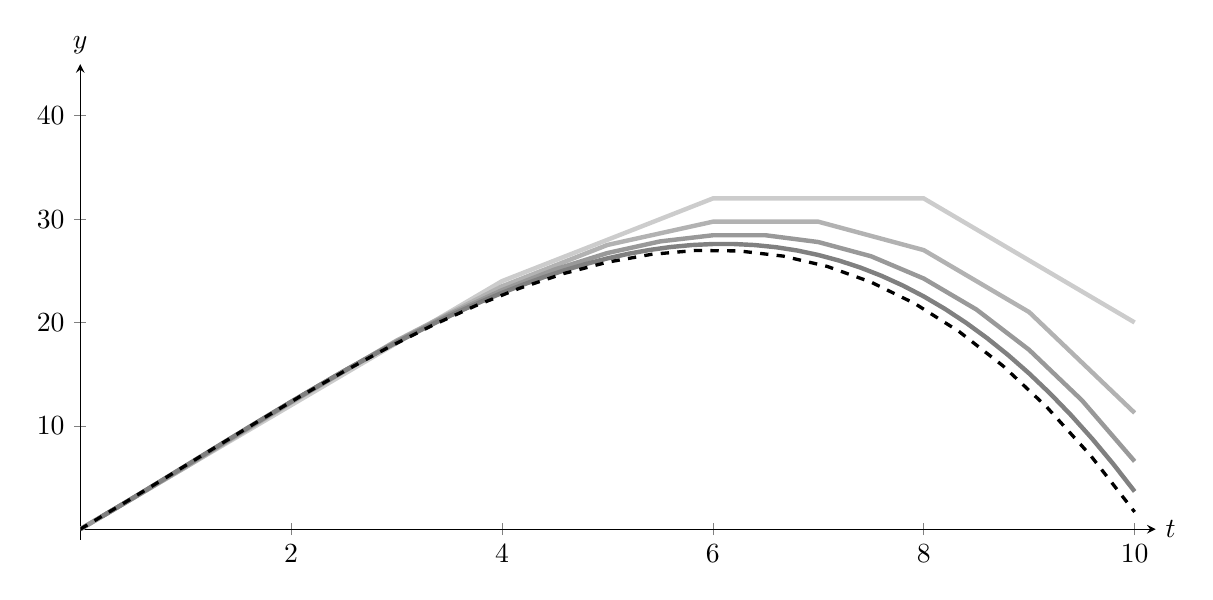
\begin{tikzpicture}[
      declare function = {f(\x) = 6+\x/2 - pow(\x,2)/4;} ]
    \begin{axis}[
        domain=0:10, xmin =0,xmax=10.2,ymax=45,ymin=-1,
        width=6in,
        height=3in,
        xtick={0,2,4,6,8,10}, 
        %xticklabels={$1$,$1.5$,$2$, $2.5$, $3$},
        %% ytick style={draw=none},
        %% yticklabels={},
        axis lines=center, xlabel=$t$, ylabel=$y$,
        every axis y label/.style={at=(current axis.above origin),anchor=south},
        every axis x label/.style={at=(current axis.right of origin),anchor=west},
      ]
      \addplot [draw=black!20!white,ultra thick] plot coordinates {(0,0) (2, 12) (4, 24) (6, 32) (8, 32) (10, 20)};
      
      \addplot [draw=black!30!white,ultra thick] plot coordinates {(0,0) (1., 6.) (2., 12.25) (3., 18.25) (4., 23.5) (5., 27.5) (6., 
        29.75) (7., 29.75) (8., 27.) (9., 21.) (10., 11.25)
      };

      \addplot [draw=black!40!white,ultra thick] plot coordinates {(0,0) (0.5, 3.) (1., 6.09375) (1.5, 9.21875) (2., 12.3125) (2.5, 
        15.3125) (3., 18.1563) (3.5, 20.7813) (4., 23.125) (4.5, 25.125) 
        (5., 26.7188) (5.5, 27.8438) (6., 28.4375) (6.5, 28.4375) (7., 
        27.7813) (7.5, 26.4063) (8., 24.25) (8.5, 21.25) (9., 17.3438) 
(9.5, 12.4688) (10., 6.5625)};
      
      
      \addplot [draw=black!50!white,ultra thick] plot coordinates {(0.2, 1.2) (0.4, 2.418) (0.6, 3.65) (0.8, 4.892) (1., 6.14) 
        (1.2, 7.39) (1.4, 8.638) (1.6, 9.88) (1.8, 11.112) (2., 12.33) 
        (2.2, 13.53) (2.4, 14.708) (2.6, 15.86) (2.8, 16.982) (3., 
        18.07) (3.2, 19.12) (3.4, 20.128) (3.6, 21.09) (3.8, 22.002) 
        (4., 22.86) (4.2, 23.66) (4.4, 24.398) (4.6, 25.07) (4.8, 
        25.672) (5., 26.2) (5.2, 26.65) (5.4, 27.018) (5.6, 27.3) (5.8, 
        27.492) (6., 27.59) (6.2, 27.59) (6.4, 27.488) (6.6, 27.28) 
        (6.8, 26.962) (7., 26.53) (7.2, 25.98) (7.4, 25.308) (7.6, 
24.51) (7.8, 23.582) (8., 22.52) (8.2, 21.32) (8.4, 19.978) 
(8.6, 18.49) (8.8, 16.852) (9., 15.06) (9.2, 13.11) (9.4, 
10.998) (9.6, 8.72) (9.8, 6.272) (10., 3.65)};
      
      \addplot [draw=black,very thick,dashed] {6*x + x^2/4-x^3/12};
    \end{axis}
  \end{tikzpicture}
\end{image}
At this point, we can explain the notation for antiderivatives. If we
``sum'' all of the ``$ds$,'' we find the value of position. Hence
\begin{align*}
  \d s &= v(t) \d t\\
  \text{``sum'' } \d s &= \text{``sum'' } v(t) \d t\\
  \int \d s &= \int v(t) \d t\\
  s(t) &= \int v(t) \d t,
\end{align*}
thus we see that an antiderivative is, essentially, a sum.
   
  
\end{document}
